\documentclass[10pt]{article}
\title{Základné meranie odporu, napätia a prúdu pomocou digitálneho multimetra}
\usepackage{blindtext}
\usepackage{geometry}
\usepackage{fancyhdr}
\usepackage{xcolor,sectsty}
\usepackage{sectsty}
\usepackage{multirow}

\usepackage{mathastext}
\usepackage{siunitx}

\usepackage[utf8]{inputenc}
\usepackage[english]{babel}

\usepackage{wrapfig}
\usepackage{hyperref}
\usepackage{graphicx}
\graphicspath{ {e:/lateximages/} }

\usepackage{pgfplots} 
\usepackage{indentfirst}

\usepackage{setspace}

\renewcommand{\baselinestretch}{1.5} 

 \geometry{
 a4paper,
 total={170mm,240mm},
 left=25mm,
 top=25mm,
 bottom=20mm,
 right=15mm
 }

\pagestyle{fancy}
\fancyhf{}
\rhead{\thepage}
\lhead{Systémy DTP}
\renewcommand{\headrulewidth}{0pt}
\renewcommand{\footrulewidth}{0pt}
\fancyfoot[C]{Zadanie č.3}
\pagestyle{empty}

\sectionfont{\fontsize{12}{15}\selectfont}

\definecolor{nadpis}{RGB}{255,99,71}
\font\myfont=cmr12 at 16pt

\title{{\myfont \color{nadpis} Základné meranie odporu, napätia a prúdu pomocou digitálneho multimetra}\vspace{9pt}}
\date{}

\begin{document}
\maketitle
\section{Niekoľko slov o digitálnom multimetri}
\textrm{\textbf{
Digitálny multimeter všeobecne nahradilmultimeter analógového typu ako testovacie zariadenie voľby pre správcov, pretože sa ľahšie číta, sú často kompaktnejšie a majú väčšiu presnosť. Digitálny multimeter vykonáva všetky štandardné analógové meracie funkcie \textcolor{blue}{\textbf{AC a DC}}. Niektoré ponúkajú meranie frekvencie a teploty.
Základné meranie odporu, napätia a prúdu pomocou digitálneho multimetra
Mnohé z nich majú také vlastnosti ako displej s vrcholom, ktorý poskytuje krátkodobú pamäť na zachytenie špičkovej hodnoty prechodových signálov, ako aj zvukových a vizuálnych indikácií na testovanie kontinuity a detekcie úrovne.
}}

\noindent\makebox[\linewidth]{\rule{\paperwidth}{0.4pt}}
\vspace{2cm}
\subsection{Odstranovanie problémov}
Pri odstraňovaní problémov s digitálnym multimeteromsprávca je schopný „vidieť“ situáciu a problém v rámci okruhu alebo systému. Obrázok 1 znázorňuje typický autoritatívny digitálny multimeter.
\begin{figure}[htbp]
\href{https://crushtymks.com/images/electrical-lectures/basic-measuring-of-resistance-voltage-and-current-using-digital-multimeter.jpg}{\includegraphics{multimeter}}
\centering
\caption{Digitálny multimeter}
\end{figure}
Samozrejme, že meradlo musí byť vždy pripojené k obvodu alebo zariadeniu, ktoré sa má testovať. Oboje vedie, jedna červená a druhá čierna, musia byť vložené do správnych konektorov vodičov. Čierny vodič je pripojený k zdierke označenej \textcolor{blue}{\textbf{COM}} alebo spoločnou.
To je zvyčajne v pravom dolnom jack, ako v tomtoilustrácie. (Uvedomte si, že nie každý meter má rovnakú konfiguráciu konektora.) Červený vodič je pripojený k niektorému z príslušných konektorov v závislosti od toho, čo chce správca merať - ohmov, voltov alebo ampérov.
Pri meraní prúdu sa používajú dva konektory na ľavej strane. buď v rozsahu \textcolor{blue}{\textbf{300 mA}} alebo \textcolor{blue}{\textbf{10 ampérov}}.
Pozrime sa teraz na základné postupy merania troch hlavných elektrických jednotiek:
\begin{itemize}
   \item[--] Odpor
   \item[--] Napätie
   \item[--] Prúd
\end{itemize}
\thispagestyle{fancy}%

\section{Meranie odporu}Obrázok 2 ukazuje kroky, ktoré treba dodržiavaťpri meraní odporu. Nezabúdajte, že merania odporu sa vykonávajú bez toho, aby bol výkon aplikovaný na testovaný komponent a hodnoty odporu sa môžu líšiť až o 20\% v dôsledku tolerancie určitých odporov.
Nenechajte sa mýliť, ak sa hodnota vášho glukometra mierne líši od farebného pásma na odpore. Ak je hodnota odporu vypnutá a presahuje toleranciu, odpor by mal byť vymenený! Rezistor bude zriedka krátky, ale typicky sa otvorí.
Ak sa rezistor otvorí, displej digitálneho multimetra bude blikať a vypínať alebo zobrazovať \textcolor{blue}{\textbf{O}}L (otvorený riadok), pretože odpor má nekonečný odpor.
\begin{enumerate}
   \item Vypnite napájanie okruhu
   \item Vyberte odpor \si{\ohm}
  \item Zapojte čierny testovací kábel do konektora COM a červený testovací kábel do konektora \si{\ohm}
  \item Špičky sondy pripojte cez komponent alebo časť obvodu, pre ktorý chcete určiť odpor
  \item Zobrazte čítanie a nezabudnite si všimnúť mernú jednotku \si{\ohm} , \si{\ohm} , M\si{\ohm}  atď. 
\end{enumerate}
\begin{figure}[htbp]
\href{https://crushtymks.com/images/electrical-lectures/basic-measuring-of-resistance-voltage-and-current-using-digital-multimeter_2.jpg}{\includegraphics{multimeter2}}
\centering
\caption{Meranie odporu}
\end{figure}
\begin{center}
\begin{table}[htbp]
\centering
\begin{tabular}{ |c|c|c|c| } 
\hline
\textbf{Svorka 1} & \textbf{Svorka 2} &\textbf{ Svorka 3} \\
\hline
\multirow{3}{4em}{$<$ 10A} & $<$ 200mA & $<$ 1A \\ 
& 100\si{\ohm} & 100k\si{\ohm} \\ 
& 20V & 300V \\
\hline
\end{tabular}
\caption{\label{tab:Tabuľka}Tabuľka hodnôt.}
\end{table}
\end{center}
Pri odstraňovaní problémov s digitálnym multimeteromsprávca je schopný vidiet situáciu a problém v rámci okruhu alebo systému. Obrázok 1 znázorňuje typický autoritatívny digitálny multimeter.
Samozrejme, že meradlo musí byť vždy pripojené k obvodu alebo zariadeniu, ktoré sa má testovať. Oboje vedie, jedna červená a druhá čierna, musia byť vložené do správnych konektorov vodičov. Čierny vodič je pripojený k zdierke označenej \textcolor{blue}{\textbf{COM}} alebo spoločnou.

\section{Meranie napätia}
\begin{wrapfigure}{r}{0.25\textwidth}
\vspace*{-0.5cm}
\href{https://crushtymks.com/images/electrical-lectures/basic-measuring-of-resistance-voltage-and-current-using-digital-multimeter_3.jpg}{\includegraphics[width=0.25\textwidth]{multimeter3}}
\centering
\caption{Meranie napätia}
\end{wrapfigure}
Obrázok 3 ukazuje kroky, ktoré by sa mali dodržiavať pri meraní napätia, Meranie napätia a odporu je tam, kde digitálny multimeter zistí najväčšie využitie.
Pri meraní napätia a odporu sa červený vodič zasunie do konektora V \si{\ohm} (volt alebo ohm).
\begin{itemize}
   \item[--] Vyberte volty AC (V), volty DC (V), mvolts (V) podľa potreby
   \item[--] Zapojte čierny testovací kábel do konektora COM a červený testovací kábel do konektora V
   \item[--] Dotknite sa hrotov sondy k obvodu naprieč záťažou alebo zdrojom napájania, ako je znázornené (paralelne s testovaným obvodom)
   \item[--] Zobrazenie čítania si určite všimnete mernú jednotku
\end{itemize}
\textcolor{blue}{\textbf{Poznámka}} // Pre hodnoty DC so správnou polaritou (+ alebo -),dotknite sa červenej testovacej sondy na kladnej strane obvodu a čiernej testovacej sondy na negatívnej strane uzemnenia obvodu. Ak zvrátite spojenia, digitálny multimeter s automatickou polaritou zobrazí len znamienko mínus označujúce zápornú polaritu. Pri analógovom merači riskujete poškodenie glukometra.

\hfill \break
\hfill \break
\hfill \break
\hfill \break
\hfill \break
\hfill \break
\hfill \break
\section{Meranie prúdu}
Obrázok 4 znázorňuje kroky, ktoré treba dodržiavať pri meraní prúdu, Meranie prúdu sa zriedka vykonáva pri odstraňovaní problémov, pretože cesta okruhu sa musí otvoriť, aby sa digitálny multimeter vložil do série s prúdovým tokom.
Ak sa však má merať prúd, červený vodič sa vloží do jedného z ampérových konektorov, 10 amp (10A) alebo 300 miliamp (300 mA) vstupný konektor v závislosti od očakávanej hodnoty čítania.
\begin{enumerate}
   \item Vypnite napájanie okruhu
   \item Odpojte, odrežte alebo odpájajte obvod, čím vytvoríte miesto, kde sa dajú vložiť sondy
   \item Podľa potreby vyberte zosilňovače AC (A) alebo zosilňovače DC (A)
   \item Zapojte čierny testovací kábel do konektora COM a červený testovací kábel do konektora 10 amp (10A) alebo 300 miliamp (300mA) v závislosti od očakávanej hodnoty čítania
   \item Pripojte hroty sondy k obvodu naprieč chlebom tak, ako je znázornené na obrázku tak, aby cez merací prístroj prúdil všetok prúd (sériové pripojenie)
   \item Zapnite napájanie obvodu
\end{enumerate}
\begin{figure}
\centering
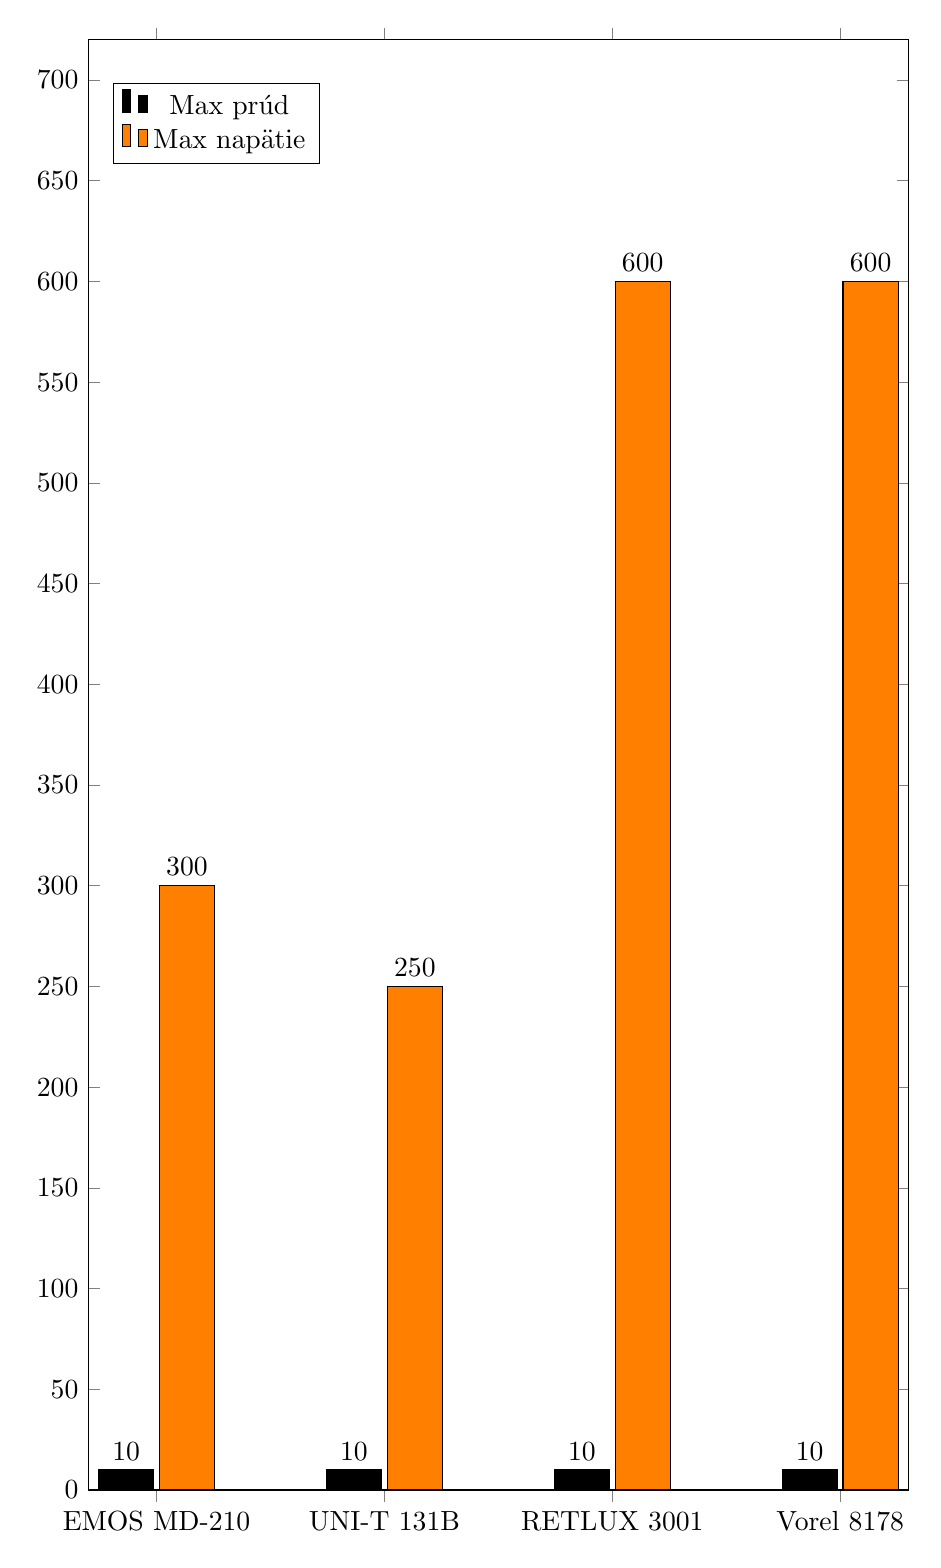
\begin{tikzpicture}
    \begin{axis}[
        ybar,
        ymin=0,
        width=12cm,
        height=20cm,
        bar width=20pt,
        nodes near coords,
        symbolic x coords={EMOS MD-210, UNI-T 131B, RETLUX 3001, Vorel 8178},
        xtick = data,
        enlarge y limits={value=0.2,upper},
        legend pos=north west
    ]
    \addplot[fill=black] coordinates {(EMOS MD-210, 10) (UNI-T 131B, 10) (RETLUX 3001, 10) (Vorel 8178, 10)};
     \addplot[fill=orange] coordinates {(EMOS MD-210, 300) (UNI-T 131B, 250) (RETLUX 3001, 600) (Vorel 8178, 600)};
      \legend{Max prúd, Max napätie}
    \end{axis}
\end{tikzpicture}
\caption{Meranie na konkrétnych multimetroch}
\label{Meranie na konkrétnych multimetroch}
\end{figure}
\end{document}